

\label{cap:3}

\section{Large Hadron Collider}
\label{par:3.1}
The Large Hadron Collider (LHC) is the world's largest and most powerful particle accelerator. It first started up on 10 September 2008, and consists of a 27-kilometre ring of superconducting magnets with a number of accelerating structures to boost the energy of the particles along the way. The LHC has a circumference of \mbox{$27$ km}. By design, its maximum achievable energies are \mbox{$7$ TeV} for beam of protons and \mbox{$2.76$ TeV} per nucleon for beam of lead ions, thus providing collisions at \mbox{$\sqrt{s}$ = $14$ TeV} and \mbox{$\sqrt{s_{NN}}$ = $5.5$ TeV}, respectively. These would be the largest energies ever achieved in particle collision experiments.


Inside the accelerator, two high-energy particle beams travel at close to the speed of light before they are made to collide. The beams travel in opposite directions in separate beam pipes - two tubes kept at ultrahigh vacuum. They are guided around the accelerator ring by a strong magnetic field maintained by superconducting electromagnets. The accelerator has to bend the beams around the ring, keep the bunches focused and accelerate them to their collision energy. Finally, the spatial dimension of the bunches has to be minimised in order to attain high luminosity, which ensure a high number of collisions per time interval at the collision points, i.e. a high luminosity\footnote{For a particle accelerator experiment, the luminosity is defined by: \mbox{$\mathcal{L} = fnN^{2}/A$} with $n$ number of bunches in both beams, $N$ number of particles per bunch, cross-sectional area $A$ of the beams that overlap completely, and revolution frequency $f$. The frequency of interactions (or in general of a given process) can be calculated from the corresponding cross-section $\sigma$ and the luminosity: \mbox{$dN/dt = \mathcal{L}\sigma$}.}. A combination of magnetic and electric field components performs the mentioned tasks. Despite the high luminosity reached, only a very small fraction of the particles of two bunches collides in a single bunch crossing. The others leave the interaction region essentially uninfluenced, are defocused, and continue to circulate in the accelerator.


Injection of bunches into the LHC (\mbox{Figure \ref{Fig:cap3-1.1}}) is preceded by acceleration in the LINAC2, PS booster, PS, and SPS accelerators. The acceleration sequence is slightly different for heavy-ions, in which case bunches pass the LINAC3, LEIR, PS, and SPS accelerators (more information can be found in \cite{LHC04}). Several injections to the LHC are needed until all bunches of both beams are filled. 

\begin{figure}[t]
\centering
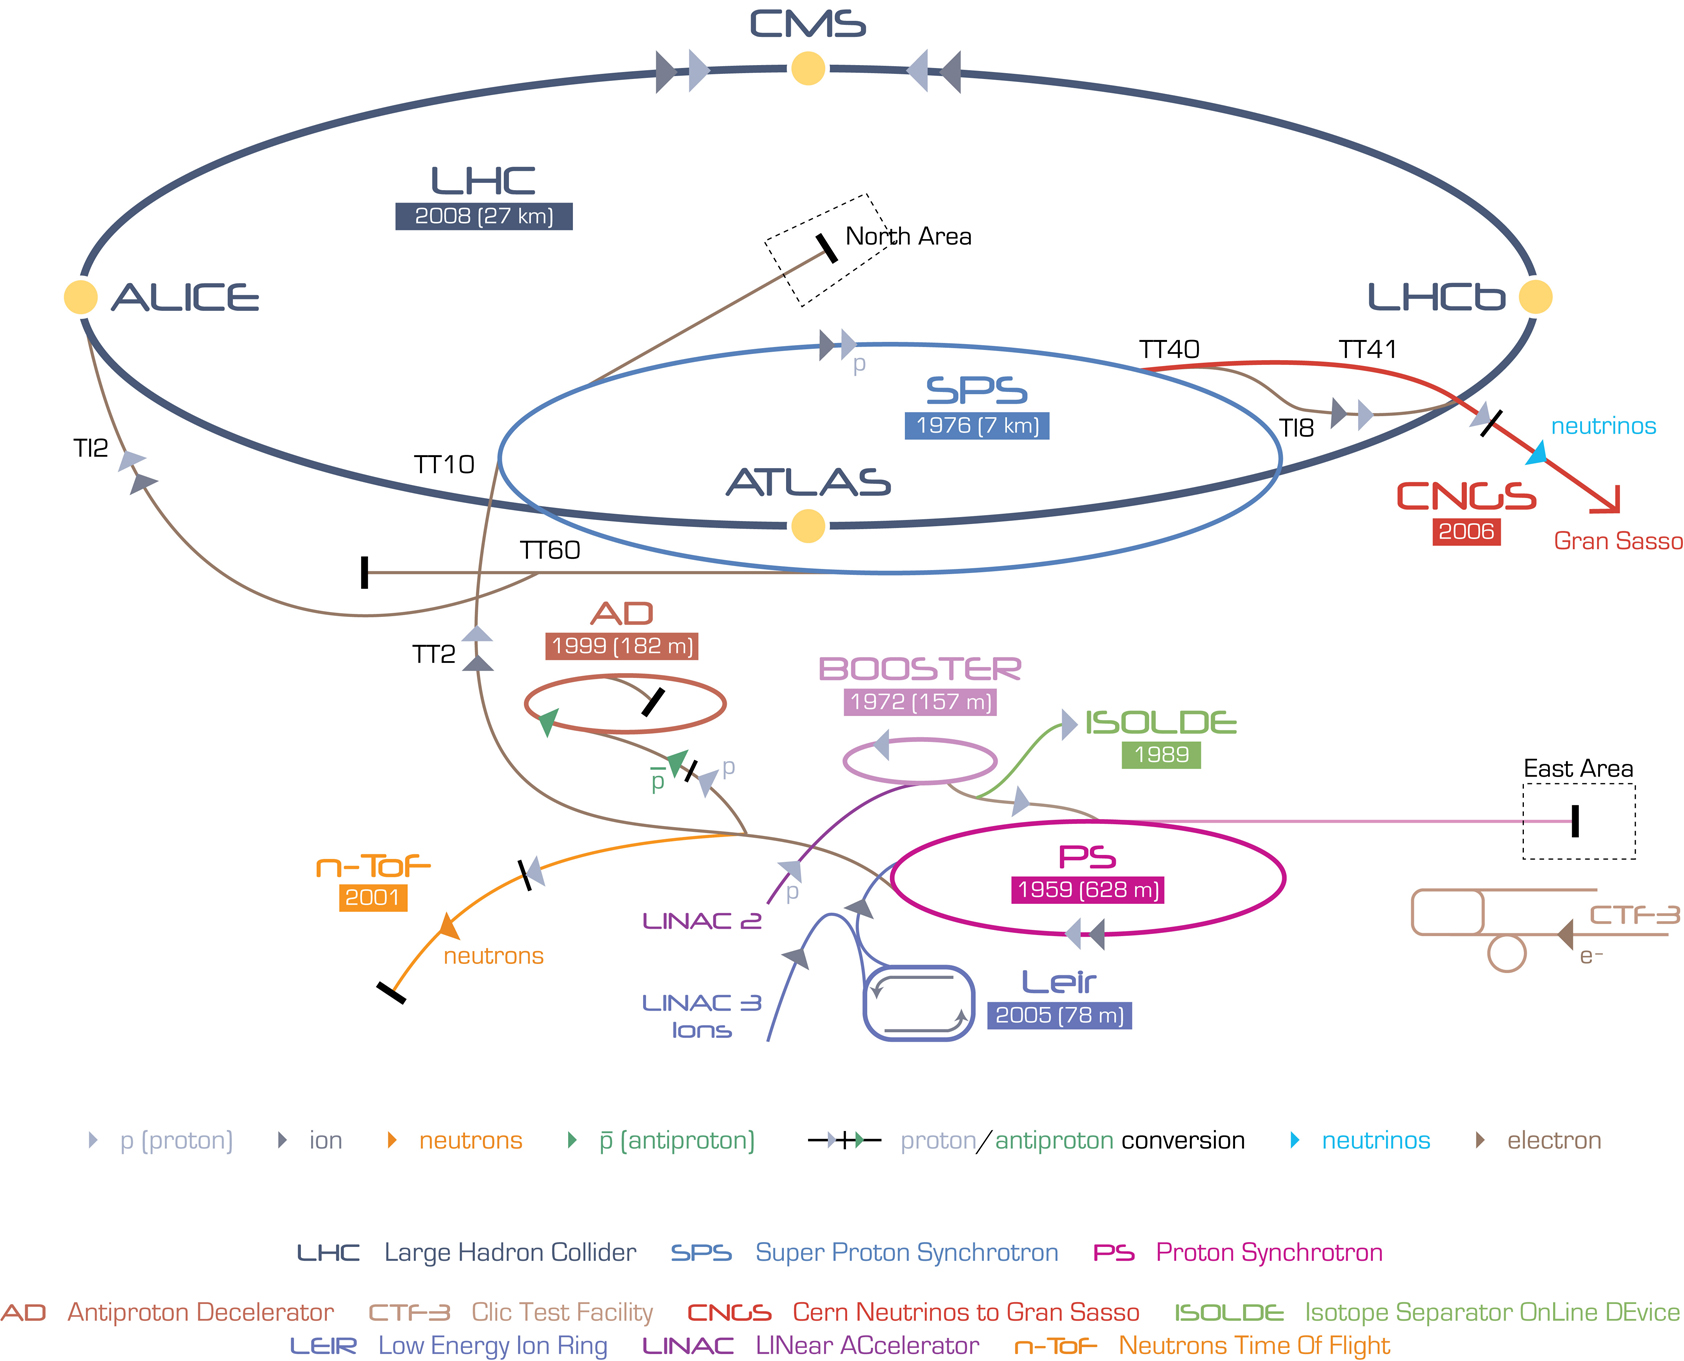
\includegraphics[width=1.0\textwidth]{Images/Cern-Accelerator-Complex}
\caption[The CERN accelerator complex.]{The CERN accelerator complex. \cite{LHC}}
\label{Fig:cap3-1.1}
\end{figure}

